%! TEX root = ../main.tex
\documentclass[main]{subfiles}

\begin{document}
\section{使用方法}

\subsection{動作する環境}

検証したOSは以下の通りです.

\begin{itemize}
    \item Windows 10
    \item macOS 10.14 or later
    \item Ubuntu 18.04 LTS or later
\end{itemize}

Dockerを利用したビルドではTeX Live 2021を用いています.その他のツールの要求バージョンは以下の通りです.

% textlint-disable ja-technical-writing/sentence-length
\begin{itemize}
    \item Docker CE 18.09 or later(Linux)
    \item Docker Desktop for Windows(Windows)
    \item Docker Desktop for Mac(macOS)
    \item GNU Make 3.8 or later
    \item (Optional) hub version 2.12.0 or later(https://github.com/github/hub)
    \item (Optional) Nodejs v14.0.0 or later
\end{itemize}
% textlint-enable ja-technical-writing/sentence-length

ただし,これは完璧に動作することを保証したものではありません.使用者の環境によっては一部機能等がうまく動作しない可能性もあります.

\subsection{論文作成時のワークフロー}

簡単に,このテンプレートを使用してどのように執筆を進めるかを示します.また,概要を図\ref{fig:workflow}に示します.

\begin{figure}[h]
    \centering
    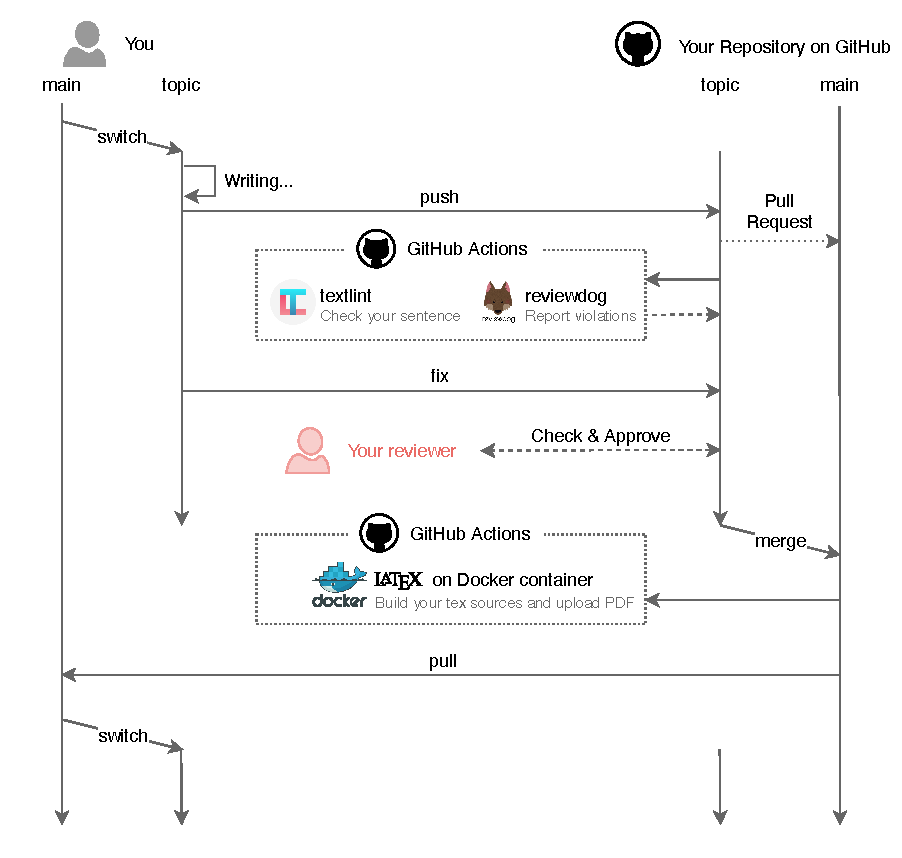
\includegraphics[keepaspectratio,scale=1.0]{../figures/textlint_workflow.pdf}
    \caption{textlintとGitHub Actionsを活用した執筆フロー}
    \label{fig:workflow}
\end{figure}

% textlint-disable ja-technical-writing/sentence-length
\begin{description}
    \item[前提] \\
        masterブランチに居る.
    \item[これからすること] \\
        新しい章を書き始める.
    \item[手順] \\
        \begin{enumerate}
            \item ブランチを切り空のPull Requestを発行する.
                \code{make draft branch=ブランチ名}で新しいブランチが切られ,
                Pull Request発行の画面がブラウザで開くので,タイトル等を入力する.
            \item 通常通りtexソースを編集してcommitおよびpush.
            \item textlintによる校正結果がreviewdogによりレビューとして投稿されるので,それを参考に修正する.
            \item ある程度書けたら共著者や教員・先輩など,内容をレビューする人をレビュアーとしてアサインする.
            \item レビュアーの指摘を元に修正.
            \item 全ての指摘を修正し,加筆の必要がなくなった時点でmasterへマージする.
            \item ローカルのリポジトリでmasterをチェックアウトしてgit pullする.
            \item 1へ戻る.
        \end{enumerate}
\end{description}
% textlint-enable ja-technical-writing/sentence-length

このイテレーションをセクションごとに行います.1つのセクションが大きい場合,その中の切りの良い単位で区切り,複数に分けて行います.1つのPull Requestによる加筆が図表等抜きで10ページを超えるようなら,変更のサイズが大きすぎるかも知れません.より小さい単位の細かいPull Requestへ分けることを推奨します.

また,一人で複数の章を同時並行で編集する場合や,複数人がそれぞれ異なる章を単一ファイルで編集する場合,容易にコンフリクトが発生し得ます.これを避けるため,大きな章ごとにsubfilesパッケージと\code{\textbackslash subfile}を使用してソースファイルを分割することを推奨します.これを使用すると,各子セクションを個別にコンパイルでき,かつ,親となるTeXソースのプリアンブルを共有する事が出来ます.構成などはこのテンプレートを参考にしてください.

\subsection{Makefileによる各種操作}

PDFの生成に関連した操作は全て,デフォルトでDockerコンテナを利用します.これは \code{USE\_DOCKER} という環境変数によって制御されています.デフォルトでは \code{USE\_DOCKER=yes} です.
Dockerは不要でネイティブで動かしたい場合,\code{USE\_DOCKER=no}とすることでこれを無効化できます.

また,Windowsで利用する場合は\lstlistingname\ref{code:powershell-env}および\lstlistingname\ref{code:cmd-env}のようにすることでDockerの有効無効を切り替えることが出来ます.

% textlint-disable ja-technical-writing/sentence-length,ja-technical-writing/no-doubled-joshi
\begin{lstlisting}[caption={Powershellの場合},label={code:powershell-env}]
    C:\Users\You> # 無効にする
    C:\Users\You> $env:USE_DOCKER="no"
    C:\Users\You> # 有効にする
    C:\Users\You> $env:USE_DOCKER="yes"
\end{lstlisting}

\begin{lstlisting}[caption={cmd.exeの場合},label={code:cmd-env}]
    C:\Users\You> rem 無効にする
    C:\Users\You> set USE_DOCKER=no
    C:\Users\You> rem 有効にする
    C:\Users\You> set USE_DOCKER=yes
\end{lstlisting}
% textlint-enable ja-technical-writing/sentence-length,ja-technical-writing/no-doubled-joshi

\subsubsection{make pdf}

main.texをコンパイルし,完全なPDFを生成するコマンドです.このコマンドでは\code{\textbackslash subfile}によって分割したファイルを個別にコンパイルすることはサポートされていません.

このツールは全体を通してコンパイルにはlatexmkを使用します.デフォルトで使用されている.latexmkrcをカスタマイズするには,\ref{sec:mklatexmkrc}をご覧ください.

\subsubsection{make watch}

latexmkによる変更検知時の自動ビルドを実行します.Dockerを利用しない場合,viewerの指定があればビルドしたPDFを開きます.Dockerを利用する場合,Dockerコンテナ内からホスト上のPDFビューワを開くことができないため,\code{-view=none}として開かないようにしています.自動リロードに対応したPDFビューワで開くと,ビルドの度に自動で変更が反映されます.


このコマンドでは分割したファイルの個別コンパイルをサポートしています.例えば以下の様に実行することで,sections/usage.texだけをusage.pdfとして閲覧できます.

\begin{lstlisting}
    $ make watch target=sections/usage.tex
\end{lstlisting}
targetの指定が無い場合,main.texを監視してコンパイルします.

\subsubsection{make all}

TeXソースのコンパイルを行う前に,前回のコンパイルによる生成物を全て破棄してコンパイルを実行します.

\subsubsection{make clean}

コンパイルによる成果物を全て破棄します.最終成果物のPDFも含めて破棄されることに注意してください.

\subsubsection{make draft}

現在のブランチから新しいブランチを切り,空のcommitを行ってリモートへpushします.その後,hubコマンドを利用してPull Request作成のページを標準のブラウザで表示します.実行時にブランチ名を指定することが出来ます.指定しない場合,デフォルト値の\code{WIP}が使用されます.

\begin{lstlisting}
    $ make draft branch=NAME
\end{lstlisting}

\subsubsection{make latexmkrc}
\label{sec:mklatexmkrc}

コンテナ内で使用されている.latexmkrcをこのディレクトリ直下にコピーします.これを編集することで,latexmkの動作をカスタマイズできます.

\subsubsection{make lint}
\label{sec:mklint}

GitHub Actions上で実行されるlintをローカルでも実行します.事前にNodejsをインストールし\code{npm install}を実行しておく必要があります.

\subsubsection{make fix}
\label{sec:mkfix}

lintに違反したもののうち,自動的に適用が可能なものについて訂正します.これは例えばprhなどによる表記揺れ訂正が対応しています.\ref{sec:mklint}と同様に,事前にNodejsのインストールと\code{npm install}の実行が必要です.

\subsection{VSCode}

このテンプレートはVSCodeで利用することを想定しています.単にVSCodeで開き,LaTeX Workshopをインストールするだけで利用可能になるようにsettings.jsonを記述しています.

\end{document}
